\documentclass[12pt]{report}
\usepackage[utf8]{inputenc}
\usepackage[english]{babel}
\usepackage{indentfirst}
\usepackage{graphicx}
\usepackage{geometry}
\usepackage[
backend=bibtex,
style=numeric,
sorting=none
]{biblatex}
\usepackage{csquotes}
\graphicspath{ {./images/} }
\addbibresource{references.bib}
\linespread{1}
\geometry{lmargin=1in, rmargin=1in, top=1in}

\title{\textbf{Heart chambers identification}}
\author{Lukacs Raul, Budur Alisa, Boitoș Roxana}

\begin{document}
\maketitle
\setlength{\parindent}{1cm}

\begin{abstract}

\end{abstract}
\tableofcontents{}

\chapter{Introduction}
\section{Motivation}
Atrial fibrillation (AF) or arrhythmia is the most common cardiac disorder encountered in clinical practice. 2.2 million people in America and 4.5 million people in Europe are affected by either paroxysmal or persistent AF \cite{sankaranarayanan1}. 

\chapter{Scientific problem}
\section{Definition}
The subject of this work it to build a method/application which is able to identify heart chamber from scans. A major advantage of this method/application is that it could assist a doctor in his job to make a correct decision. Also, it could be even a learning tool for medical school student. It would teach them where are the chambers in a heart scan.

Identification of heart chambers from MRI scans reduces, in terms of computer science, to a classification problem. We have to classify pixels in two classes: those that belong to a heart chamber and the others.  In order to solve this, there are two steps:

\begin{enumerate}
	\item Extract the region of interest from the scan - this is an image containing only the heart, no other bones or other organs. Then, for each pixel of the image, get the color and brightness;
	\item  Use a supervised learning algorithm to classify the pixels. Input of the algorithm is color of the pixel and output is a boolean value, \textit{true} meaning that the pixel is part of a hear chamber and  \textit{false} meaning that the pixel is not part of a heart chamber.
\end{enumerate}

This is a very interesting problem to solve because it implies a good knowledge of heart anatomy, as well as good knowledge of machine learning algorithms. 

\chapter{Related work}
This paper \cite{bai1} describes a method to do left ventricular myocardium segmentation using multi-altas segmentation. In order to archive this the paper proposes two novel segmentation algorithms, PBAF and SVMAF, which incorporate gradient and contextual information into multi-atlas label fusion. The dataset used were randomly selected from the DETERMINE (Defibrillators to Reduce Risk by Magnetic Resonance Imaging Evaluation) study the contains MR images from patients with coronary artery disease and regional wall motion abnormalities due to prior myocardial infarction. Experimental results on a short-axis cardiac MR data set of 83 subjects have demonstrated that the accuracy of multi-atlas segmentation can be significantly improved by using the augmented feature vector.

This paper \cite{gomez1} presents a benchmark of current algorithms that segment the left atrium (LA) from  Computed Tomography(CT) and  Magnetic Resonance Imaging(MRI) datasets. The used datasets provide a variety of quality levels in the following proportions: 8 high contrast, 15 moderate contrast, 3 low contrast and 4 high noise datasets for CT datasets  and 9 high quality, 10 moderate quality, 6 local artefacts and 5 high noise datasets for MRI datasets. A standardization framework for left atrial surfaces was implemented  to reduce the influence of inconsistently defined regions. The ground truth and automatic segmentations were standardized. Using the framework, the boundaries of the LA were consistently identified on all datasets. The paper presents the results of  for nine algorithms for CT and eight algorithms for MRI. Results showed that algorithms combining an atlas/model based approach with a region growing approach perform best in segmenting the left atrium from CT and MRI datasets.

\chapter{Proposed approach}

Our approach is to use two supervised learning algorithms to solve this problem. First algorithm is an artificial neural network (ANN). We have chosen this one because it is a universal function approximators for non-linear functions \cite{annAdvantages}. Also, it is easy to use understand. Second algorithm is a support vector machine (SVM) We have chosen this one because it can provide good results being trained even with an unbalanced dataset (one class has more items than the other.)

\section{Description of artificial neural network with back-propagation learning}
 \subsection{Feed-forward artificial neural network}
 \subsubsection{Structure}
 An artificial neural network contains multiple nodes connected by links. Each link has an associated weight. Actually, learning is done by updating these weights. “\textit{In a layered feed-forward network, each unit is linked only to units in the next layer; there are no links between units in the same layer, no links backward to a previous layer, and no links that skip a layer}"  \cite{artificialIntelligenceModernApproach}.
 
 \subsubsection{How it works}
 Each unit performs a simple computation: it receives signals from its input links and computes a new activation level that it sends along each of its output links. The computation is split into two components. First, it computes the weighted sum of the unit's input values. Second, it applies the activation function to the wighted sum.  Usually, all units in a network use the same activation function.
 
 \subsubsection{Back-propagation learning}
 Learning in a feed-forward neural network is performed in the following way: inputs are presented to the network and it computes an output vector. Then, an error is computed  (the difference between the output and target). If the error is zero, nothing happens. Otherwise, the weights are adjusted to  reduce this error. The challenge is to divide the error among the contributing weights. The back-propagation algorithm is an approach to dividing the contribution of each weight. See an example below in figure \ref{fig:back-propagation}.
 
 \begin{figure}[h]
 	\centering
 	\fbox{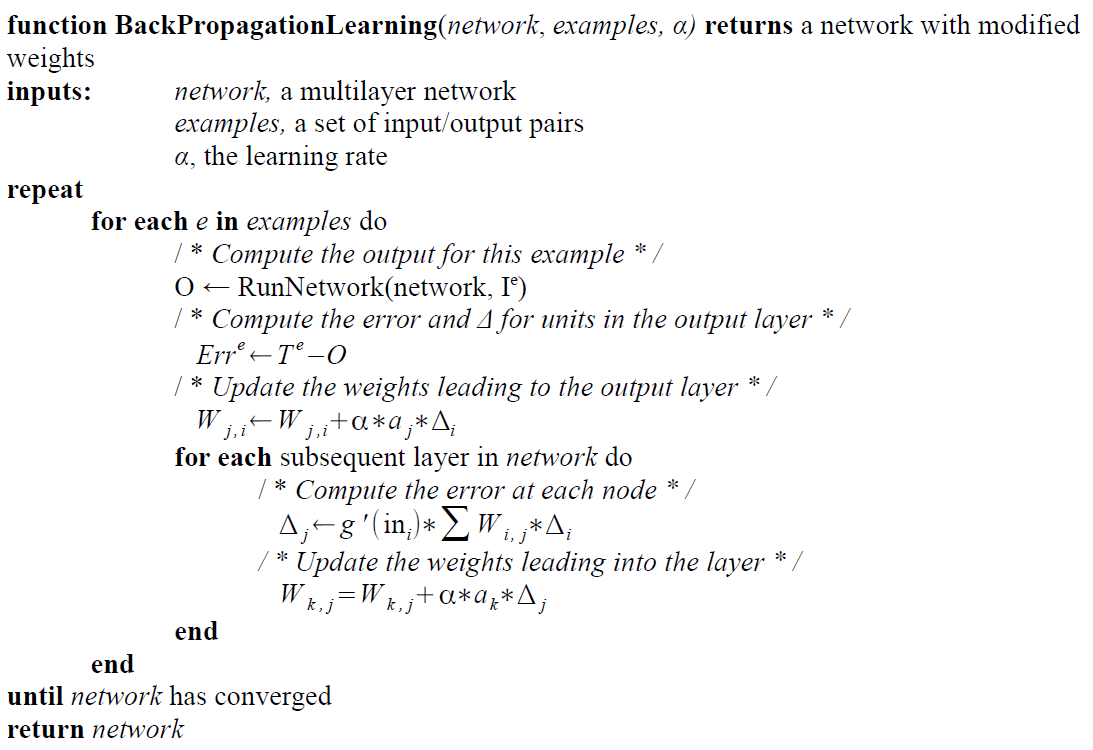
\includegraphics[width=0.8\linewidth]{images/back-propagation}}
 	\caption{Back-propagation learning algorithm}
 	\label{fig:back-propagation}
 \end{figure}

\chapter{Application}
\section{Methodology}
We created an application that can identify all heart chambers from MRI scans. In order to achieve this, we trained an artificial neural network to learn how to identify heart chambers. For training, we used heart MRI scans: the original image pixels (as input) and the labeled image (as output).

The hyper-parameters used for of neural network were: 
\begin{enumerate}
	\item minimum error: 0.01;
	\item learning rate: 0.1;
	\item number of epochs: 1000;
	\item number of hidden layers: 2;
	\item number of neurons in input layer: 6400;
	\item number of neurons in output layer: 6400.
\end{enumerate}  

Before training the algorithm, we normalized the input images in two steps: first, we resized all images to be 80x80 pixels; then, for each image we created an array with all pixels from the image and then we normalized that array to have values in the interval [0, 1], using the following formula: 
\begin{equation}
x_{normalized}=\frac{x_{i} - x_{min}}{x_{max} - x_{min}}
\end{equation}

After normalizing the array, we used it as input for the artificial neural network algorithm. The output of the algorithm was interpreted in the following way: if the neuron value is greater or equal to 0.5, then that neuron represents a pixel that belongs to the object. Otherwise, that pixel belongs to the background. 

\section{Data}
We used MRI scans provided by Boston Children's Hospital \cite{dataSet}. The images are 3D cardiovascular magnetic resonance images and some of them include a congenital heart defects. Imaging was done in an axial view on a 1.5T scanner (Phillips Achieva) without contrast agent using a steady-state free precession (SSFP) pulse sequence. Manual segmentation of the blood pool and ventricular myocardium was performed by a trained rater, and validated by two clinical experts. We used 30 images from this dataset.

\section{Results}
For validating the machine learning algorithm, we used cross-validation method with k = 10: we chose 27 (90\%) images for training and 3 (10\%) for testing. We train and test the algorithm 10 times and compute the mean accuracy value, which was: 62.82\%. That means that 62.82\% of pixels were classified correctly.

\section{Discussion}
We consider that the accuracy value, which was not very high, was due to the fact that we used a small amount of training data. We know that one major disadvantage of artificial neural networks is that they require a large amount of training data.

\printbibliography
\end{document}
